% Options for packages loaded elsewhere
\PassOptionsToPackage{unicode}{hyperref}
\PassOptionsToPackage{hyphens}{url}
%
\documentclass[
]{book}
\usepackage{lmodern}
\usepackage{amssymb,amsmath}
\usepackage{ifxetex,ifluatex}
\ifnum 0\ifxetex 1\fi\ifluatex 1\fi=0 % if pdftex
  \usepackage[T1]{fontenc}
  \usepackage[utf8]{inputenc}
  \usepackage{textcomp} % provide euro and other symbols
\else % if luatex or xetex
  \usepackage{unicode-math}
  \defaultfontfeatures{Scale=MatchLowercase}
  \defaultfontfeatures[\rmfamily]{Ligatures=TeX,Scale=1}
\fi
% Use upquote if available, for straight quotes in verbatim environments
\IfFileExists{upquote.sty}{\usepackage{upquote}}{}
\IfFileExists{microtype.sty}{% use microtype if available
  \usepackage[]{microtype}
  \UseMicrotypeSet[protrusion]{basicmath} % disable protrusion for tt fonts
}{}
\makeatletter
\@ifundefined{KOMAClassName}{% if non-KOMA class
  \IfFileExists{parskip.sty}{%
    \usepackage{parskip}
  }{% else
    \setlength{\parindent}{0pt}
    \setlength{\parskip}{6pt plus 2pt minus 1pt}}
}{% if KOMA class
  \KOMAoptions{parskip=half}}
\makeatother
\usepackage{xcolor}
\IfFileExists{xurl.sty}{\usepackage{xurl}}{} % add URL line breaks if available
\IfFileExists{bookmark.sty}{\usepackage{bookmark}}{\usepackage{hyperref}}
\hypersetup{
  pdftitle={DMAC Training Modules},
  pdfauthor={Kyle Roell, Lauren Koval, Julia Rager},
  hidelinks,
  pdfcreator={LaTeX via pandoc}}
\urlstyle{same} % disable monospaced font for URLs
\usepackage{color}
\usepackage{fancyvrb}
\newcommand{\VerbBar}{|}
\newcommand{\VERB}{\Verb[commandchars=\\\{\}]}
\DefineVerbatimEnvironment{Highlighting}{Verbatim}{commandchars=\\\{\}}
% Add ',fontsize=\small' for more characters per line
\usepackage{framed}
\definecolor{shadecolor}{RGB}{248,248,248}
\newenvironment{Shaded}{\begin{snugshade}}{\end{snugshade}}
\newcommand{\AlertTok}[1]{\textcolor[rgb]{0.94,0.16,0.16}{#1}}
\newcommand{\AnnotationTok}[1]{\textcolor[rgb]{0.56,0.35,0.01}{\textbf{\textit{#1}}}}
\newcommand{\AttributeTok}[1]{\textcolor[rgb]{0.77,0.63,0.00}{#1}}
\newcommand{\BaseNTok}[1]{\textcolor[rgb]{0.00,0.00,0.81}{#1}}
\newcommand{\BuiltInTok}[1]{#1}
\newcommand{\CharTok}[1]{\textcolor[rgb]{0.31,0.60,0.02}{#1}}
\newcommand{\CommentTok}[1]{\textcolor[rgb]{0.56,0.35,0.01}{\textit{#1}}}
\newcommand{\CommentVarTok}[1]{\textcolor[rgb]{0.56,0.35,0.01}{\textbf{\textit{#1}}}}
\newcommand{\ConstantTok}[1]{\textcolor[rgb]{0.00,0.00,0.00}{#1}}
\newcommand{\ControlFlowTok}[1]{\textcolor[rgb]{0.13,0.29,0.53}{\textbf{#1}}}
\newcommand{\DataTypeTok}[1]{\textcolor[rgb]{0.13,0.29,0.53}{#1}}
\newcommand{\DecValTok}[1]{\textcolor[rgb]{0.00,0.00,0.81}{#1}}
\newcommand{\DocumentationTok}[1]{\textcolor[rgb]{0.56,0.35,0.01}{\textbf{\textit{#1}}}}
\newcommand{\ErrorTok}[1]{\textcolor[rgb]{0.64,0.00,0.00}{\textbf{#1}}}
\newcommand{\ExtensionTok}[1]{#1}
\newcommand{\FloatTok}[1]{\textcolor[rgb]{0.00,0.00,0.81}{#1}}
\newcommand{\FunctionTok}[1]{\textcolor[rgb]{0.00,0.00,0.00}{#1}}
\newcommand{\ImportTok}[1]{#1}
\newcommand{\InformationTok}[1]{\textcolor[rgb]{0.56,0.35,0.01}{\textbf{\textit{#1}}}}
\newcommand{\KeywordTok}[1]{\textcolor[rgb]{0.13,0.29,0.53}{\textbf{#1}}}
\newcommand{\NormalTok}[1]{#1}
\newcommand{\OperatorTok}[1]{\textcolor[rgb]{0.81,0.36,0.00}{\textbf{#1}}}
\newcommand{\OtherTok}[1]{\textcolor[rgb]{0.56,0.35,0.01}{#1}}
\newcommand{\PreprocessorTok}[1]{\textcolor[rgb]{0.56,0.35,0.01}{\textit{#1}}}
\newcommand{\RegionMarkerTok}[1]{#1}
\newcommand{\SpecialCharTok}[1]{\textcolor[rgb]{0.00,0.00,0.00}{#1}}
\newcommand{\SpecialStringTok}[1]{\textcolor[rgb]{0.31,0.60,0.02}{#1}}
\newcommand{\StringTok}[1]{\textcolor[rgb]{0.31,0.60,0.02}{#1}}
\newcommand{\VariableTok}[1]{\textcolor[rgb]{0.00,0.00,0.00}{#1}}
\newcommand{\VerbatimStringTok}[1]{\textcolor[rgb]{0.31,0.60,0.02}{#1}}
\newcommand{\WarningTok}[1]{\textcolor[rgb]{0.56,0.35,0.01}{\textbf{\textit{#1}}}}
\usepackage{longtable,booktabs}
% Correct order of tables after \paragraph or \subparagraph
\usepackage{etoolbox}
\makeatletter
\patchcmd\longtable{\par}{\if@noskipsec\mbox{}\fi\par}{}{}
\makeatother
% Allow footnotes in longtable head/foot
\IfFileExists{footnotehyper.sty}{\usepackage{footnotehyper}}{\usepackage{footnote}}
\makesavenoteenv{longtable}
\usepackage{graphicx,grffile}
\makeatletter
\def\maxwidth{\ifdim\Gin@nat@width>\linewidth\linewidth\else\Gin@nat@width\fi}
\def\maxheight{\ifdim\Gin@nat@height>\textheight\textheight\else\Gin@nat@height\fi}
\makeatother
% Scale images if necessary, so that they will not overflow the page
% margins by default, and it is still possible to overwrite the defaults
% using explicit options in \includegraphics[width, height, ...]{}
\setkeys{Gin}{width=\maxwidth,height=\maxheight,keepaspectratio}
% Set default figure placement to htbp
\makeatletter
\def\fps@figure{htbp}
\makeatother
\setlength{\emergencystretch}{3em} % prevent overfull lines
\providecommand{\tightlist}{%
  \setlength{\itemsep}{0pt}\setlength{\parskip}{0pt}}
\setcounter{secnumdepth}{5}
\usepackage{booktabs}
\usepackage[]{natbib}
\bibliographystyle{plainnat}

\title{DMAC Training Modules}
\author{Kyle Roell, Lauren Koval, Julia Rager}
\date{2021-06-23}

\begin{document}
\maketitle

{
\setcounter{tocdepth}{1}
\tableofcontents
}
\hypertarget{introduction}{%
\chapter{Introduction}\label{introduction}}

The \href{https://sph.unc.edu/superfund-pages/srp/}{UNC-Superfund Research Program} (SRP) seeks to develop new solutions for reducing exposure to inorganic arsenic and prevent arsenic-induced diabetes through mechanistic and translational research.

The \href{https://sph.unc.edu/superfund-pages/dmac/}{Data Analysis and Management Core} (DMAC) provide the UNC-Superfund Research Program with critical expertise in bioinformatics, statistics, data management and data integration. Our goal is to support the data management, integration, and analysis needs of the researchers to reveal multi-factorial determinants of inorganic arsenic-induced metabolic dysfunction/diabetes.

All code for these modules can be found at the \href{https://github.com/UNCSRP}{UNC-SRP Github Page}.


\includegraphics[width=45.58in]{_book/test1_files/figure-html/SRP_logo}

\hypertarget{intro}{%
\chapter{Setting Up Your R Environment}\label{intro}}

Before learning about data manipulation and statistical methods for analyzing environmental health datasets, we will provide a brief introduction to R, RStudio, and setting up an R environment and simple scripts.

\hypertarget{r-and-rstudio}{%
\section{R and RStudio}\label{r-and-rstudio}}

\href{https://www.r-project.org}{R} is a free, open source programming language for statistical computing and graphics that anyone can download and use. It doesn't require a license and is good for reproducible analyses. There exists a large, diverse collection of packages and very comprehensive documentation.

It is easy to download, install, and setup R. Additionally, \href{https://www.rstudio.com}{RStudio} is an open source integrated development environment for R. RStudio makes programming in R and using R scripts and features more user friendly. R should be downloaded prior to downloading RStudio.

\hypertarget{downloading-r-and-rstudio}{%
\subsection{Downloading R and RStudio}\label{downloading-r-and-rstudio}}

The following is a walkthrough on how to download R and RStudio.

\textbf{1. Navigate to R Website}

\begin{figure}
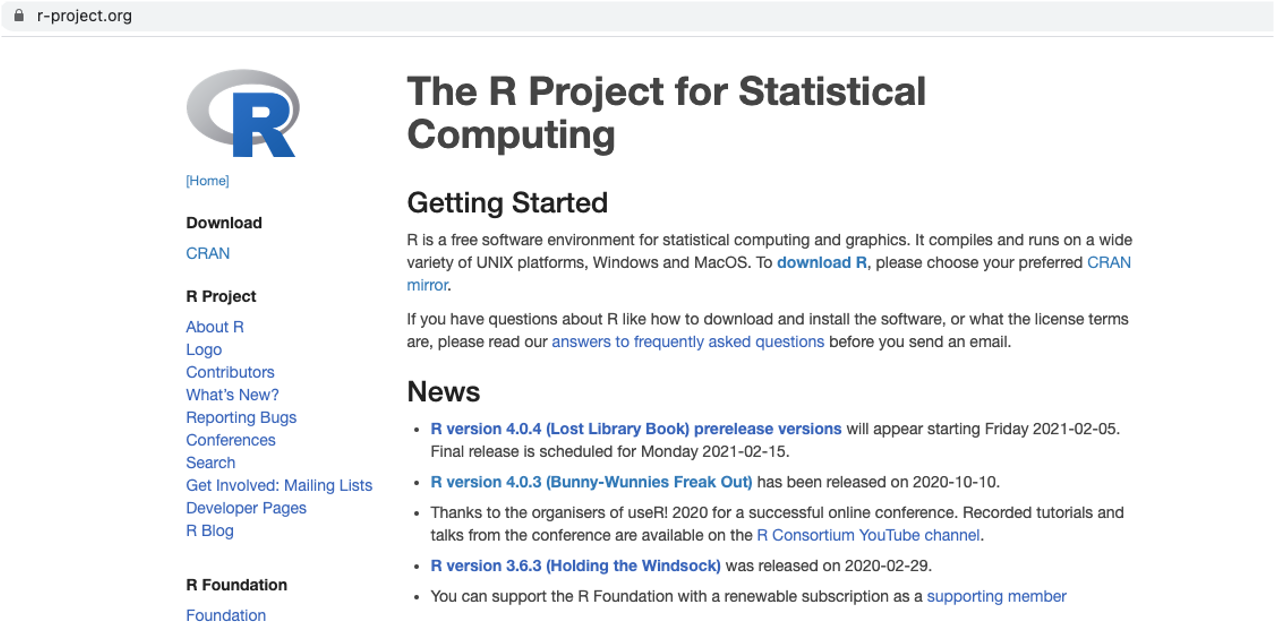
\includegraphics[width=17.71in]{_book/test1_files/figure-html/r_website} \caption{R Website, https://www.r-project.org}\label{fig:website}
\end{figure}

\textbf{2. Select the appropriate CRAN mirror (Duke is fastest if at UNC)}

\begin{figure}
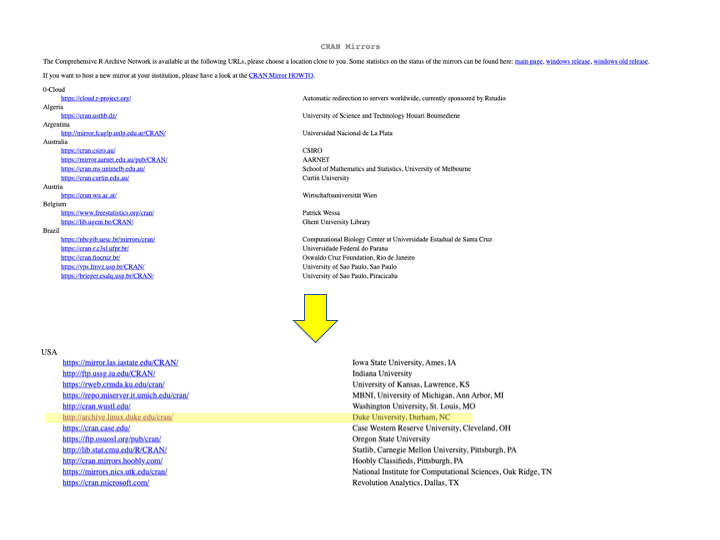
\includegraphics[width=17.85in]{_book/test1_files/figure-html/cran_mirrors} \caption{CRAN Mirror, https://cran.r-project.org/mirrors.html}\label{fig:mirror}
\end{figure}

\textbf{3. Select the appropriate R distribution}

\begin{figure}
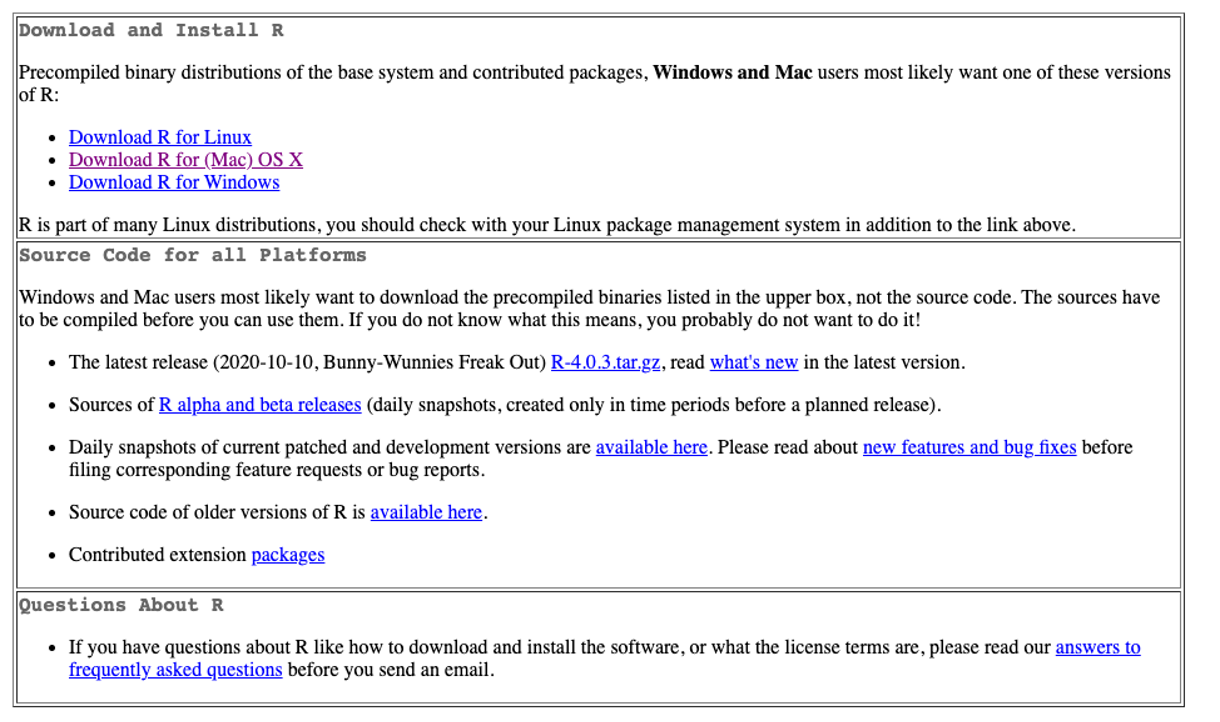
\includegraphics[width=16.94in]{_book/test1_files/figure-html/duke_archive_r} \caption{R Download Link, http://archive.linux.duke.edu/cran/}\label{fig:archive}
\end{figure}

\textbf{4. Download R}

\begin{figure}
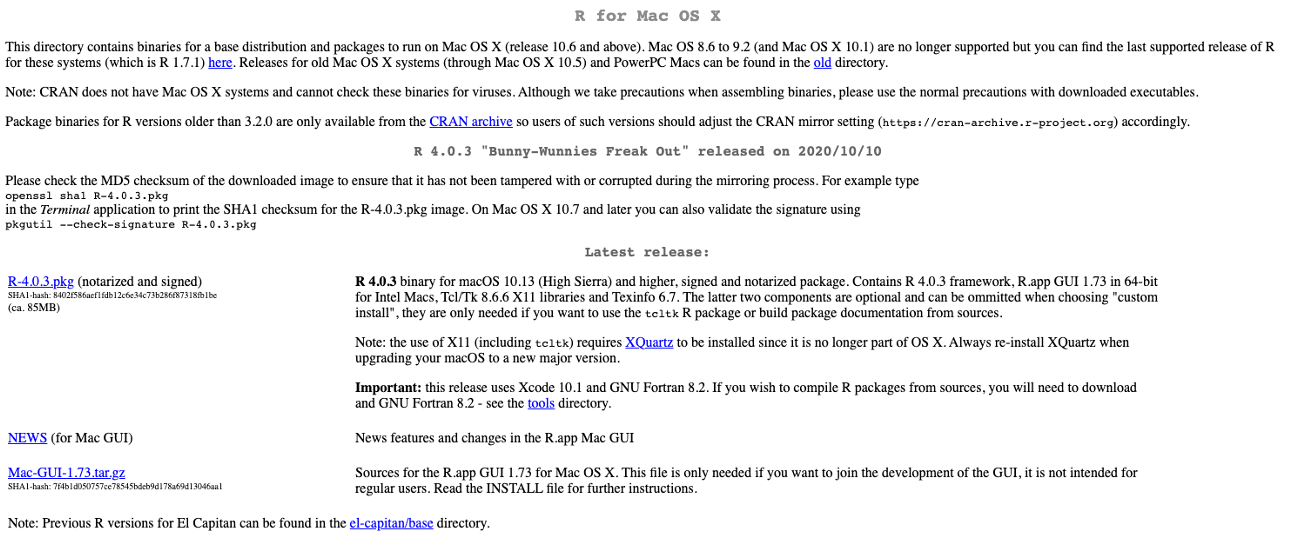
\includegraphics[width=17.93in]{_book/test1_files/figure-html/duke_download_r} \caption{R Download, http://archive.linux.duke.edu/cran/bin/macosx/}\label{fig:download}
\end{figure}

\textbf{5. Navigate to RStudio website and download RStudio (free edition)}

\begin{figure}
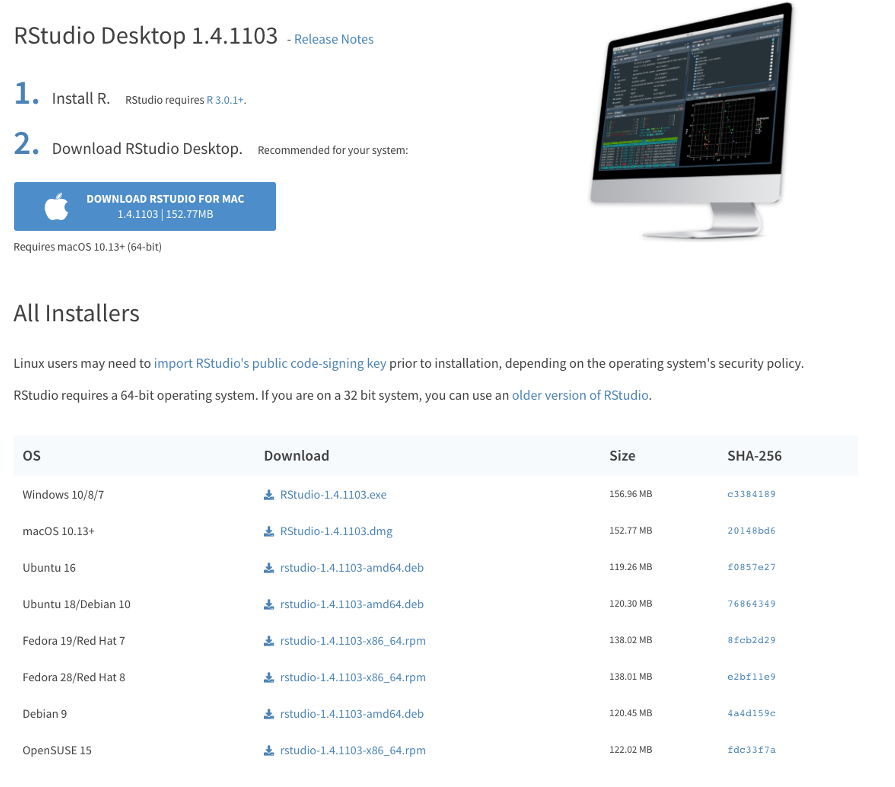
\includegraphics[width=12.43in]{_book/test1_files/figure-html/rstudio} \caption{RStudio Download, https://rstudio.com/products/rstudio/download/}\label{fig:downloadstudio}
\end{figure}

\hypertarget{installing-r-and-rstudio}{%
\subsection{Installing R and RStudio}\label{installing-r-and-rstudio}}

Once R and RStudio have been downloaded, install R first and then RStudio, following the instructions of the installer.

\hypertarget{installing-and-loading-packages}{%
\subsection{Installing and Loading Packages}\label{installing-and-loading-packages}}

Packages in R are units of shareable code that contain functions, data, and documentation on how to use all of these resources. Because R is an open source programming language, packages are constantly being developed and updated. There are many R packages that exist spanning many topics such as graphics and plotting, machine learning, and data manipulation. R packages are often written by R users and submitted to the \href{https://cran.r-project.org}{Comprehensive R Archive Network} (CRAN), or another host such as \href{https://www.bioconductor.org}{BioConductor} or \href{https://github.com}{GitHub}.

Packages can be installed from the host, but need to be loaded into the workspace. Most of the time, you do not need to download anything from a website. Instead, you can install packages through running code in R or RStudio.

\begin{Shaded}
\begin{Highlighting}[]
\KeywordTok{install.packages}\NormalTok{(}\StringTok{"ggplot2"}\NormalTok{, }\DataTypeTok{repos =} \StringTok{"https://cran.rstudio.com"}\NormalTok{)}
\end{Highlighting}
\end{Shaded}

Once a package is installed, it needs to be loaded using the \emph{library} function or explicitly referenced to use functions or datasets from that package.

\begin{Shaded}
\begin{Highlighting}[]
\KeywordTok{library}\NormalTok{(ggplot2)}
\end{Highlighting}
\end{Shaded}

\hypertarget{scripting-basics}{%
\section{Scripting Basics}\label{scripting-basics}}

Before demonstrating the basics of writing R code and scripts, it is worth noting that a function can be queried in RStudio by typing a question mark before the name of the function (e.g.~\emph{?install.packages}). This will bring up documentation in the viewer window. Additionally, RStudio will autofill function names, variable names, etc. by pressing tab while typing. If multiple matches are found, RStudio will provide you with a drop down list to select from, which may be useful when searching through newly installed packages or trying to quickly type variable names in an R script.

R also allows for scripts to contain non-code elements, called comments, that will not be run or interpreted. To make a comment, simply use a \# followed by the comment. A \# only comments out a single line of code, i.e.~only that line will not be run. Comments are useful to help make code more interpretable for others or to add reminders of what and why parts of code may have been written.

\begin{Shaded}
\begin{Highlighting}[]
\CommentTok{# This is an R comment!}

\CommentTok{# Loading ggplot2 package}
\KeywordTok{library}\NormalTok{(ggplot2)}
\end{Highlighting}
\end{Shaded}

\hypertarget{setting-working-directory}{%
\subsection{Setting Working Directory}\label{setting-working-directory}}

When working in R, it can be helpful to set the working directory to a local directory where data are located or output files will be saved. The current working directory can also be displayed.

\begin{Shaded}
\begin{Highlighting}[]
\CommentTok{# Show current working directory}
\KeywordTok{getwd}\NormalTok{()}
\end{Highlighting}
\end{Shaded}

\begin{verbatim}
## [1] "/Users/kroell/Documents/IEHS/UNC-SRP/test1"
\end{verbatim}

\begin{Shaded}
\begin{Highlighting}[]
\CommentTok{# Set working directory}
\KeywordTok{setwd}\NormalTok{(}\StringTok{"~/Documents/UNCSRP/Data/"}\NormalTok{)}
\end{Highlighting}
\end{Shaded}

\hypertarget{importing-and-exporting-files}{%
\subsection{Importing and Exporting Files}\label{importing-and-exporting-files}}

After setting the working directory, importing and exporting files can be done using various functions based on the type of file being read or written. Often, it is easiest to import data into R that are in a comma separated values, comma delimited, (CSV) file or tab delimited file. Other datatypes such as SAS data files, large csv files, etc. may require different functions to be more efficienlty read in and some of these file formats will be discussed in future modules.

\begin{Shaded}
\begin{Highlighting}[]
\CommentTok{# Read in CSV data}
\NormalTok{csv.dataset =}\StringTok{ }\KeywordTok{read.csv}\NormalTok{(}\DataTypeTok{file=}\StringTok{"~/Documents/UNCSRP/Data/example_data.csv"}\NormalTok{)}

\CommentTok{# Read in tab delimited data}
\NormalTok{tab.dataset =}\StringTok{ }\KeywordTok{read.table}\NormalTok{(}\DataTypeTok{file=}\StringTok{"~/Documents/UNCSRP/Data/example_data.txt"}\NormalTok{)}
\end{Highlighting}
\end{Shaded}

There are many ways to export data in R. Data can be written out into a CSV file, tab delimited file, RData file, etc. There are also many functions within packages that write out specific datasets generated by that package.

\begin{Shaded}
\begin{Highlighting}[]
\CommentTok{# Write out to a CSV file}
\KeywordTok{write.csv}\NormalTok{(csv.output, }\DataTypeTok{file=}\StringTok{"~/Documents/UNCSRP/Output/csv_output.csv"}\NormalTok{)}

\CommentTok{# Write out to a tab delimited file}
\KeywordTok{write.table}\NormalTok{(tab.output, }\DataTypeTok{file=}\StringTok{"~/Documents/UNCSRP/Output/tsv_output.txt"}\NormalTok{, }\DataTypeTok{sep=}\StringTok{"}\CharTok{\textbackslash{}t}\StringTok{"}\NormalTok{)}
\end{Highlighting}
\end{Shaded}

R also allows objects to be saved in RData files. These files can be read into R, as well, and will load the object into the current workspace. Entire workspaces are also able to be saved.

\begin{Shaded}
\begin{Highlighting}[]
\CommentTok{# Read in saved single R data object}
\NormalTok{r.obj =}\StringTok{ }\KeywordTok{readRDS}\NormalTok{(}\DataTypeTok{file=}\StringTok{"~/Documents/UNCSRP/Data/data.rds"}\NormalTok{)}

\CommentTok{# Write single R object to file}
\KeywordTok{saveRDS}\NormalTok{(object, }\DataTypeTok{file=}\StringTok{"~/Documents/UNCSRP/Output/single_object.rds"}\NormalTok{)}

\CommentTok{# Read in multiple saved R objects}
\KeywordTok{load}\NormalTok{(}\DataTypeTok{file=}\StringTok{"~/Documents/UNCSRP/Data/multiple_data.RData"}\NormalTok{)}

\CommentTok{# Save multiple R objects}
\KeywordTok{save}\NormalTok{(object1, object2, }\DataTypeTok{file=}\StringTok{"~/Documents/UNCSRP/Output/multiple_objects.RData"}\NormalTok{)}

\CommentTok{# Save entire workspace}
\KeywordTok{save.image}\NormalTok{(}\DataTypeTok{file=}\StringTok{"~/Documents/UNCSRP/Output/entire_workspace.RData"}\NormalTok{)}

\CommentTok{# Load entire workspace}
\KeywordTok{load}\NormalTok{(}\DataTypeTok{file=}\StringTok{"~/Documents/UNCSRP/Data/entire_workspace.RData"}\NormalTok{)}
\end{Highlighting}
\end{Shaded}

\hypertarget{viewing-data}{%
\subsection{Viewing Data}\label{viewing-data}}

After data has been loaded into R, or created within R, it is good to inspect it. Datasets can be viewed in their entirety or subset to quickly look at part of the data.

\begin{Shaded}
\begin{Highlighting}[]
\CommentTok{# View first 5 rows of the previously loaded dataset}
\NormalTok{csv.dataset[}\DecValTok{1}\OperatorTok{:}\DecValTok{5}\NormalTok{,]}
\end{Highlighting}
\end{Shaded}

\begin{verbatim}
##    Sample Var1 Var2 Var3
## 1 sample1    1    2    1
## 2 sample2    2    4    4
## 3 sample3    3    6    9
## 4 sample4    4    8   16
## 5 sample5    5   10   25
\end{verbatim}

\begin{Shaded}
\begin{Highlighting}[]
\CommentTok{# View the entire dataset in RStudio}
\KeywordTok{View}\NormalTok{(csv.dataset)}
\end{Highlighting}
\end{Shaded}

\hypertarget{dataorg}{%
\chapter{The Basics for Data Organization}\label{dataorg}}

One of the first things that is useful to learn about is data organization and manipulation. While this will not be a complete guide, as there are many things you can do in R to manipulate your data, hopefully this will get you started and will provide you with the fundamentals for working with data in R.

\hypertarget{basic-data-manipulation}{%
\section{Basic Data Manipulation}\label{basic-data-manipulation}}

Data manipulation generally refers to organizing and formatting data in a way that makes it easier to read and work with. This can be done through base R operations and functions or through a collection of packages (and philosophy) known as \href{https://www.tidyverse.org}{Tidyverse}.

In this brief tutorial we will first go over the basic operations and functions you can use to manipulate data, and then show the exact same steps using the Tidyverse packages, functions, and syntax.

\hypertarget{merging}{%
\subsection{Merging}\label{merging}}

Here, we will be looking at merging as the joining together of two or more datasets, connected using a common identifier, generally some sort of ID. This is useful if you various datasets describing different variables across the same participants. In our example, we will be joining demographic data and environmental exposure data.

\begin{Shaded}
\begin{Highlighting}[]
\CommentTok{#First, let's read in our datasets}
\NormalTok{demo.data =}\StringTok{ }\KeywordTok{read.csv}\NormalTok{(}\StringTok{"~/Downloads/demo_data.csv"}\NormalTok{);}
\NormalTok{chem.data =}\StringTok{ }\KeywordTok{read.csv}\NormalTok{(}\StringTok{"~/Downloads/chem_data.csv"}\NormalTok{);}

\CommentTok{#We can merge these by their shared ID column}
\NormalTok{full.data =}\StringTok{ }\KeywordTok{merge}\NormalTok{(demo.data, chem.data, }\DataTypeTok{by=}\StringTok{"ID"}\NormalTok{)}

\CommentTok{#We could also merge by different ID columns using: by.x = "ID.Demo", by.y="ID.Chem"}
\end{Highlighting}
\end{Shaded}

\hypertarget{filtering-subsetting}{%
\subsection{Filtering \& subsetting}\label{filtering-subsetting}}

Filtering and subsetting data is useful when you need to restrict your dataset to samples or participants with specific conditions. It is also useful for simply removing particular variables or samples.

\begin{Shaded}
\begin{Highlighting}[]
\CommentTok{#Let's define a vector of columns we want to keep}
\NormalTok{subset.columns =}\StringTok{ }\KeywordTok{c}\NormalTok{(}\StringTok{"BMI"}\NormalTok{, }\StringTok{"MAge"}\NormalTok{, }\StringTok{"MEdu"}\NormalTok{);}

\CommentTok{#Now we can simply subset our data using those columns}
\NormalTok{subset.data1 =}\StringTok{ }\NormalTok{full.data[,subset.columns];}

\CommentTok{#If we want to remove those columns, need to identify which columns need removing}
\NormalTok{remove.columns =}\StringTok{ }\KeywordTok{colnames}\NormalTok{(full.data) }\OperatorTok\StringTok{ }\NormalTok{subset.columns;}
\KeywordTok{cat}\NormalTok{(remove.columns);}
\end{Highlighting}
\end{Shaded}

\begin{verbatim}
## FALSE TRUE TRUE TRUE FALSE FALSE FALSE FALSE FALSE FALSE FALSE FALSE
\end{verbatim}

\begin{Shaded}
\begin{Highlighting}[]
\CommentTok{#Now we can subset our dataset by only keeping those that we didn't specify}
\NormalTok{subset.data1a =}\StringTok{ }\NormalTok{full.data[,}\OperatorTok{!}\NormalTok{remove.columns];}

\CommentTok{#It is easy to subset data based on rows}
\CommentTok{#Keeping only first 100 rows}
\NormalTok{subset.data2 =}\StringTok{ }\NormalTok{full.data[}\DecValTok{1}\OperatorTok{:}\DecValTok{100}\NormalTok{,];}
\CommentTok{#Removing the first 100 rows}
\NormalTok{subset.data2a =}\StringTok{ }\NormalTok{full.data[}\OperatorTok{-}\KeywordTok{c}\NormalTok{(}\DecValTok{1}\OperatorTok{:}\DecValTok{100}\NormalTok{),];}

\CommentTok{#We can also filter data using conditional statements}
\NormalTok{subset.data3 =}\StringTok{ }\NormalTok{full.data[}\KeywordTok{which}\NormalTok{(full.data}\OperatorTok{$}\NormalTok{BMI }\OperatorTok{>}\StringTok{ }\DecValTok{25} \OperatorTok{&}\StringTok{ }\NormalTok{full.data}\OperatorTok{$}\NormalTok{MAge }\OperatorTok{>}\StringTok{ }\DecValTok{31}\NormalTok{),];}
\KeywordTok{head}\NormalTok{(subset.data3);}
\end{Highlighting}
\end{Shaded}

\begin{verbatim}
##    ID      BMI     MAge     MEdu       BW       GA     DWAs      DWCd     DWCr
## 4   4 30.09710 34.81796 3.760030 3266.844 18.60876 5.906656 2.0752589 50.92745
## 5   5 37.41737 42.68440 4.484686 3664.088 32.57351 7.181873 2.7626433 55.16882
## 9   9 36.94794 33.58589 3.242318 3260.482 37.37241 9.074928 2.7277549 55.72826
## 13 13 33.65870 33.82961 2.924433 3481.293 33.68744 7.101634 0.8443918 47.11677
## 22 22 25.68414 37.08028 2.704409 3387.046 52.48203 7.207447 2.8088453 48.08648
## 31 31 28.39896 47.85761 6.453362 3173.033 20.10080 6.032807 2.1929549 45.71856
##          UAs        UCd      UCr
## 4   8.719123  0.9364825 42.47987
## 5   9.436559  1.4977829 47.78528
## 9  10.818153  1.6585757 42.58577
## 13  9.967185 -0.3466431 36.74220
## 22  9.446643  1.9891049 34.16921
## 31  9.917588  1.1194851 37.82297
\end{verbatim}

\begin{Shaded}
\begin{Highlighting}[]
\CommentTok{#This can also be done using the subset function}
\NormalTok{subset.data4 =}\StringTok{ }\KeywordTok{subset}\NormalTok{(full.data, BMI }\OperatorTok{>}\StringTok{ }\DecValTok{25} \OperatorTok{&}\StringTok{ }\NormalTok{MAge }\OperatorTok{>}\StringTok{ }\DecValTok{31}\NormalTok{);}

\CommentTok{#Additionally, we can subset and select only specific columns to keep}
\NormalTok{subset.data4 =}\StringTok{ }\KeywordTok{subset}\NormalTok{(full.data, BMI }\OperatorTok{<}\StringTok{ }\DecValTok{22} \OperatorTok{|}\StringTok{ }\NormalTok{BMI }\OperatorTok{>}\StringTok{ }\DecValTok{27}\NormalTok{, }\DataTypeTok{select=}\KeywordTok{c}\NormalTok{(}\StringTok{"BMI"}\NormalTok{, }\StringTok{"MAge"}\NormalTok{, }\StringTok{"MEdu"}\NormalTok{));}
\end{Highlighting}
\end{Shaded}

\hypertarget{melt-and-cast}{%
\subsection{Melt and Cast}\label{melt-and-cast}}

Melting and casting refers to coverting data to ``long'' or ``wide'' form. Generally, our data is in wide format, but long format is necessary for some procedures, such as plotting with \href{https://ggplot2.tidyverse.org}{ggplot2}.

\begin{Shaded}
\begin{Highlighting}[]
\CommentTok{#Melt and cast functions from reshape2 package}
\KeywordTok{library}\NormalTok{(reshape2);}

\CommentTok{#Melting data converts it to long format}
\CommentTok{#Here, we are saying we want a row for each sample (ID) and each column }
\NormalTok{full.melted =}\StringTok{ }\KeywordTok{melt}\NormalTok{(full.data, }\DataTypeTok{id=}\StringTok{"ID"}\NormalTok{)}
\CommentTok{#Let's look at the new data}
\KeywordTok{head}\NormalTok{(full.melted);}
\end{Highlighting}
\end{Shaded}

\begin{verbatim}
##   ID variable    value
## 1  1      BMI 27.69249
## 2  2      BMI 26.79125
## 3  3      BMI 33.23209
## 4  4      BMI 30.09710
## 5  5      BMI 37.41737
## 6  6      BMI 33.28761
\end{verbatim}

\begin{Shaded}
\begin{Highlighting}[]
\CommentTok{#Casting puts data into wide format}
\CommentTok{#We are telling the cast function to give us a sample (ID) }
\CommentTok{#for every variable in the variable column}
\NormalTok{full.cast =}\StringTok{ }\KeywordTok{dcast}\NormalTok{(full.melted, ID }\OperatorTok{~}\StringTok{ }\NormalTok{variable);}
\KeywordTok{head}\NormalTok{(full.cast);}
\end{Highlighting}
\end{Shaded}

\begin{verbatim}
##   ID      BMI     MAge     MEdu       BW       GA     DWAs     DWCd     DWCr
## 1  1 27.69249 22.99928 3.136759 3180.058 31.79569 6.426464 1.292941 51.67987
## 2  2 26.79125 30.05142 2.656019 3210.823 53.34991 7.832384 1.798535 50.10409
## 3  3 33.23209 28.04660 3.259116 3311.551 53.60599 7.516569 1.288461 48.74001
## 4  4 30.09710 34.81796 3.760030 3266.844 18.60876 5.906656 2.075259 50.92745
## 5  5 37.41737 42.68440 4.484686 3664.088 32.57351 7.181873 2.762643 55.16882
## 6  6 33.28761 24.94960 3.596075 3328.988 38.12531 9.723429 3.054057 51.14812
##         UAs       UCd      UCr
## 1 10.192695 0.7537104 42.60187
## 2 11.815088 0.9789506 41.30757
## 3 10.079057 0.1903262 36.47716
## 4  8.719123 0.9364825 42.47987
## 5  9.436559 1.4977829 47.78528
## 6 11.589403 1.6645837 38.26386
\end{verbatim}

\hypertarget{tidyverse}{%
\subsection{Tidyverse}\label{tidyverse}}

\href{https://www.tidyverse.org}{Tidyverse} is a collection of packages that are used together along with a specific type of syntax, dataset and formatting protocols, etc.

Here, we will peform all the of the previous exercises using Tidyverse!

\begin{Shaded}
\begin{Highlighting}[]
\KeywordTok{library}\NormalTok{(tidyverse);}

\CommentTok{#Merging}
\NormalTok{full.tidy =}\StringTok{ }\KeywordTok{inner_join}\NormalTok{(demo.data, chem.data, }\DataTypeTok{by=}\StringTok{"ID"}\NormalTok{); }

\CommentTok{#To merge with different IDs use: by = c("ID.Demo"="ID.Chem")}

\CommentTok{#Susbetting columns}
\NormalTok{subset.tidy1 =}\StringTok{ }\NormalTok{full.tidy }\OperatorTok\StringTok{ }\KeywordTok{select}\NormalTok{(}\KeywordTok{all_of}\NormalTok{(subset.columns));}
\NormalTok{subset.columns1 =}\StringTok{ }\KeywordTok{c}\NormalTok{(subset.columns, }\StringTok{"NotAColName"}\NormalTok{);}
\NormalTok{subset.tidy1a =}\StringTok{ }\NormalTok{full.tidy }\OperatorTok\StringTok{ }\KeywordTok{select}\NormalTok{(}\KeywordTok{any_of}\NormalTok{(subset.columns1));}

\CommentTok{#Removing columns}
\NormalTok{subset.tidy1b =}\StringTok{ }\NormalTok{full.tidy }\OperatorTok\StringTok{ }\KeywordTok{select}\NormalTok{(}\OperatorTok{-}\NormalTok{subset.columns);}

\CommentTok{#Susbetting Rows}
\NormalTok{subset.tidy2a =}\StringTok{ }\NormalTok{full.tidy }\OperatorTok\StringTok{ }\KeywordTok{slice}\NormalTok{(}\DecValTok{1}\OperatorTok{:}\DecValTok{100}\NormalTok{);}
\NormalTok{subset.tidy2b =}\StringTok{ }\NormalTok{full.tidy }\OperatorTok\StringTok{ }\KeywordTok{slice}\NormalTok{(}\OperatorTok{-}\KeywordTok{c}\NormalTok{(}\DecValTok{1}\OperatorTok{:}\DecValTok{100}\NormalTok{));}

\CommentTok{#Filtering data}
\NormalTok{subset.tidy3 =}\StringTok{ }\NormalTok{full.tidy }\OperatorTok\StringTok{ }\KeywordTok{filter}\NormalTok{(BMI }\OperatorTok{>}\StringTok{ }\DecValTok{25} \OperatorTok{&}\StringTok{ }\NormalTok{MAge }\OperatorTok{>}\StringTok{ }\DecValTok{31}\NormalTok{);}
\KeywordTok{head}\NormalTok{(subset.tidy3);}
\end{Highlighting}
\end{Shaded}

\begin{verbatim}
##   ID      BMI     MAge     MEdu       BW       GA     DWAs      DWCd     DWCr
## 1  4 30.09710 34.81796 3.760030 3266.844 18.60876 5.906656 2.0752589 50.92745
## 2  5 37.41737 42.68440 4.484686 3664.088 32.57351 7.181873 2.7626433 55.16882
## 3  9 36.94794 33.58589 3.242318 3260.482 37.37241 9.074928 2.7277549 55.72826
## 4 13 33.65870 33.82961 2.924433 3481.293 33.68744 7.101634 0.8443918 47.11677
## 5 22 25.68414 37.08028 2.704409 3387.046 52.48203 7.207447 2.8088453 48.08648
## 6 31 28.39896 47.85761 6.453362 3173.033 20.10080 6.032807 2.1929549 45.71856
##         UAs        UCd      UCr
## 1  8.719123  0.9364825 42.47987
## 2  9.436559  1.4977829 47.78528
## 3 10.818153  1.6585757 42.58577
## 4  9.967185 -0.3466431 36.74220
## 5  9.446643  1.9891049 34.16921
## 6  9.917588  1.1194851 37.82297
\end{verbatim}

\begin{Shaded}
\begin{Highlighting}[]
\NormalTok{subset.tidy4 =}\StringTok{ }\NormalTok{full.tidy }\OperatorTok\StringTok{ }\KeywordTok{filter}\NormalTok{(BMI }\OperatorTok{>}\StringTok{ }\DecValTok{25} \OperatorTok{&}\StringTok{ }\NormalTok{MAge }\OperatorTok{>}\StringTok{ }\DecValTok{31}\NormalTok{) }\OperatorTok\StringTok{ }\KeywordTok{select}\NormalTok{(BMI, MAge, MEdu);}

\CommentTok{#Melting and Casting (pivoting in Tidyverse)}
\NormalTok{full.pivotlong =}\StringTok{ }\NormalTok{full.tidy }\OperatorTok\StringTok{ }\KeywordTok{pivot_longer}\NormalTok{(}\OperatorTok{-}\NormalTok{ID, }\DataTypeTok{names_to =} \StringTok{"var"}\NormalTok{, }\DataTypeTok{values_to =} \StringTok{"value"}\NormalTok{);}
\KeywordTok{head}\NormalTok{(full.pivotlong, }\DecValTok{15}\NormalTok{);}
\end{Highlighting}
\end{Shaded}

\begin{verbatim}
## # A tibble: 15 x 3
##       ID var      value
##    <int> <chr>    <dbl>
##  1     1 BMI     27.7  
##  2     1 MAge    23.0  
##  3     1 MEdu     3.14 
##  4     1 BW    3180.   
##  5     1 GA      31.8  
##  6     1 DWAs     6.43 
##  7     1 DWCd     1.29 
##  8     1 DWCr    51.7  
##  9     1 UAs     10.2  
## 10     1 UCd      0.754
## 11     1 UCr     42.6  
## 12     2 BMI     26.8  
## 13     2 MAge    30.1  
## 14     2 MEdu     2.66 
## 15     2 BW    3211.
\end{verbatim}

\begin{Shaded}
\begin{Highlighting}[]
\NormalTok{full.pivotwide =}\StringTok{ }\NormalTok{full.pivotlong }\OperatorTok\StringTok{ }\KeywordTok{pivot_wider}\NormalTok{(}\DataTypeTok{names_from =} \StringTok{"var"}\NormalTok{, }\DataTypeTok{values_from=}\StringTok{"value"}\NormalTok{);}
\KeywordTok{head}\NormalTok{(full.pivotwide);}
\end{Highlighting}
\end{Shaded}

\begin{verbatim}
## # A tibble: 6 x 12
##      ID   BMI  MAge  MEdu    BW    GA  DWAs  DWCd  DWCr   UAs   UCd   UCr
##   <int> <dbl> <dbl> <dbl> <dbl> <dbl> <dbl> <dbl> <dbl> <dbl> <dbl> <dbl>
## 1     1  27.7  23.0  3.14 3180.  31.8  6.43  1.29  51.7 10.2  0.754  42.6
## 2     2  26.8  30.1  2.66 3211.  53.3  7.83  1.80  50.1 11.8  0.979  41.3
## 3     3  33.2  28.0  3.26 3312.  53.6  7.52  1.29  48.7 10.1  0.190  36.5
## 4     4  30.1  34.8  3.76 3267.  18.6  5.91  2.08  50.9  8.72 0.936  42.5
## 5     5  37.4  42.7  4.48 3664.  32.6  7.18  2.76  55.2  9.44 1.50   47.8
## 6     6  33.3  24.9  3.60 3329.  38.1  9.72  3.05  51.1 11.6  1.66   38.3
\end{verbatim}

\hypertarget{finding-and-visualizing-data-trends}{%
\chapter{Finding and Visualizing Data Trends}\label{finding-and-visualizing-data-trends}}

\hypertarget{basic-statistical-tests-and-visualizations-of-data}{%
\section{Basic Statistical Tests and Visualizations of Data}\label{basic-statistical-tests-and-visualizations-of-data}}

Need an example dataset -- maybe ELGAN shuffled/deidentified, with made-up environmental exposure column?

\hypertarget{normality}{%
\subsection{Normality}\label{normality}}

Many statistical tests and methods rely on assumptions of normality. There are a few ways to look at the normality of a dataset, both formally and informally. Plotting data using historgrams, densities, or qqplots, can graphically help inform if a variable is normally distributed. There also exist statistical tests, such as the Kolmogorov-Smirnov (K-S) normality test and Shapiro-Wilk's test, that will formally test if data come from a normal distribution. When using these tests, it is important to remember that the null hypothesis is that the sample distribution is normal, and a significant p-value means the distribution is non-normal.

Even when using more formal statistical tests to test for normality, it is important to visualize the data, as well.

\begin{Shaded}
\begin{Highlighting}[]
\CommentTok{#Histograms to visualize data}
\KeywordTok{hist}\NormalTok{(full.data}\OperatorTok{$}\NormalTok{BMI);}
\end{Highlighting}
\end{Shaded}

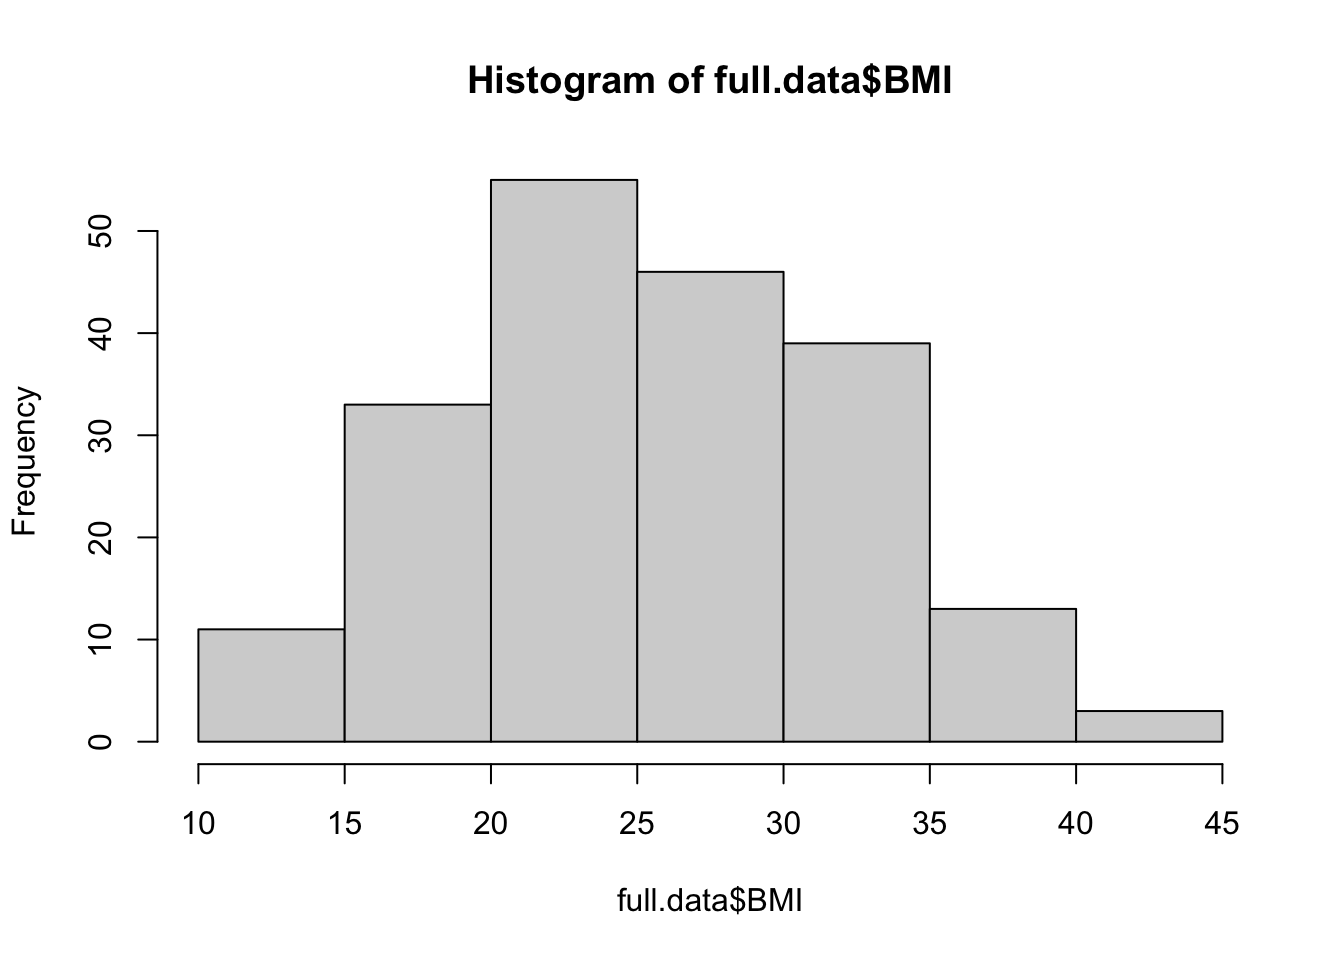
\includegraphics{test1_files/figure-latex/normality-1.pdf}

\begin{Shaded}
\begin{Highlighting}[]
\CommentTok{#Can decrease bin size (using breaks parameter) to better visualize}
\KeywordTok{hist}\NormalTok{(full.data}\OperatorTok{$}\NormalTok{BMI, }\DataTypeTok{breaks=}\DecValTok{20}\NormalTok{);}
\end{Highlighting}
\end{Shaded}

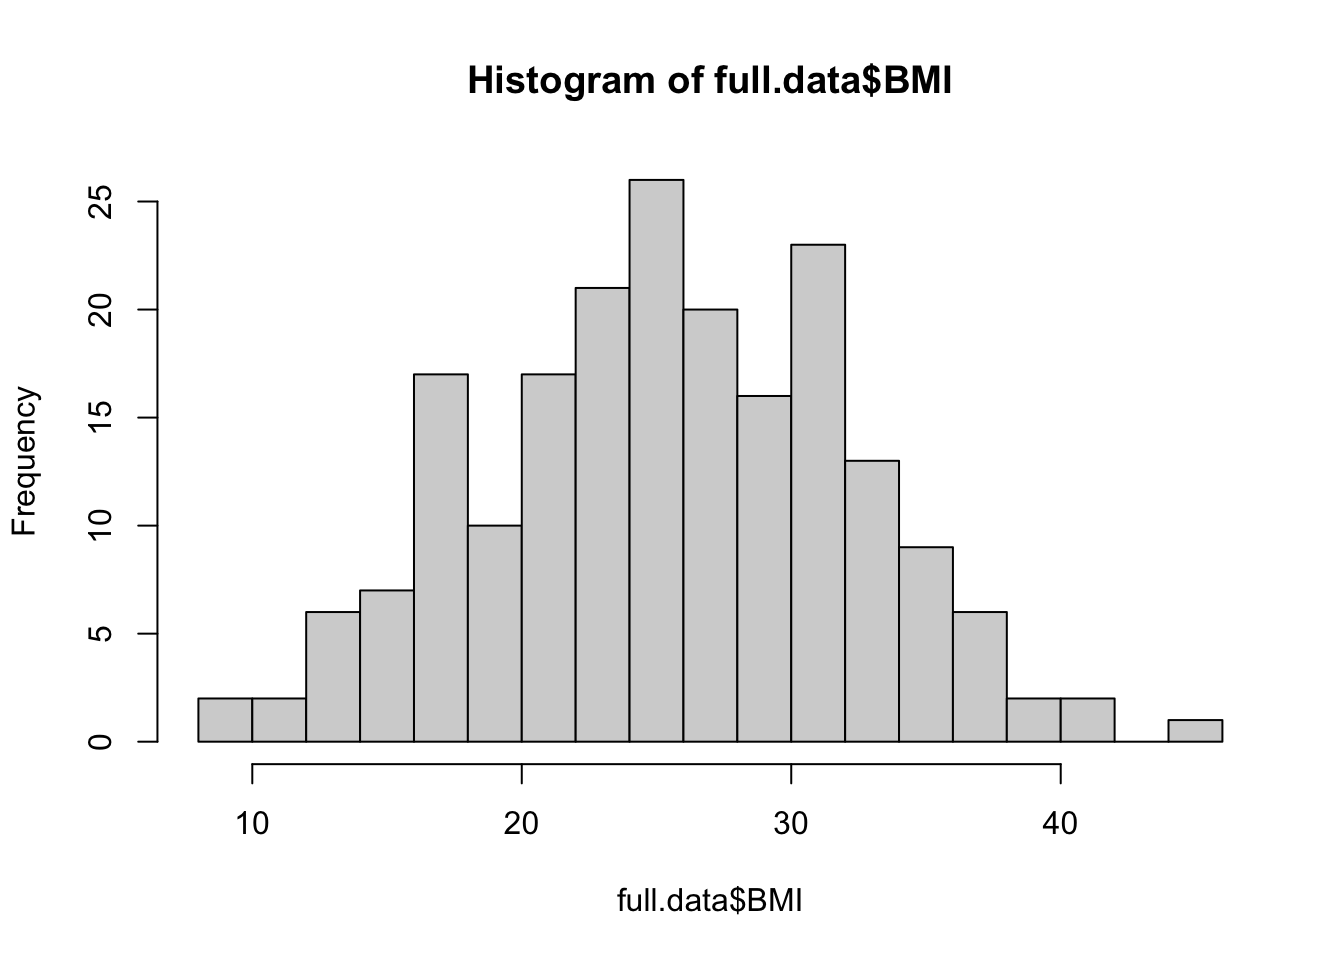
\includegraphics{test1_files/figure-latex/normality-2.pdf}

\begin{Shaded}
\begin{Highlighting}[]
\CommentTok{#Also look at normal qqplot using qqnorm function }
\KeywordTok{qqnorm}\NormalTok{(full.data}\OperatorTok{$}\NormalTok{BMI);}
\CommentTok{#Add reference line}
\KeywordTok{qqline}\NormalTok{(full.data}\OperatorTok{$}\NormalTok{BMI);}
\end{Highlighting}
\end{Shaded}

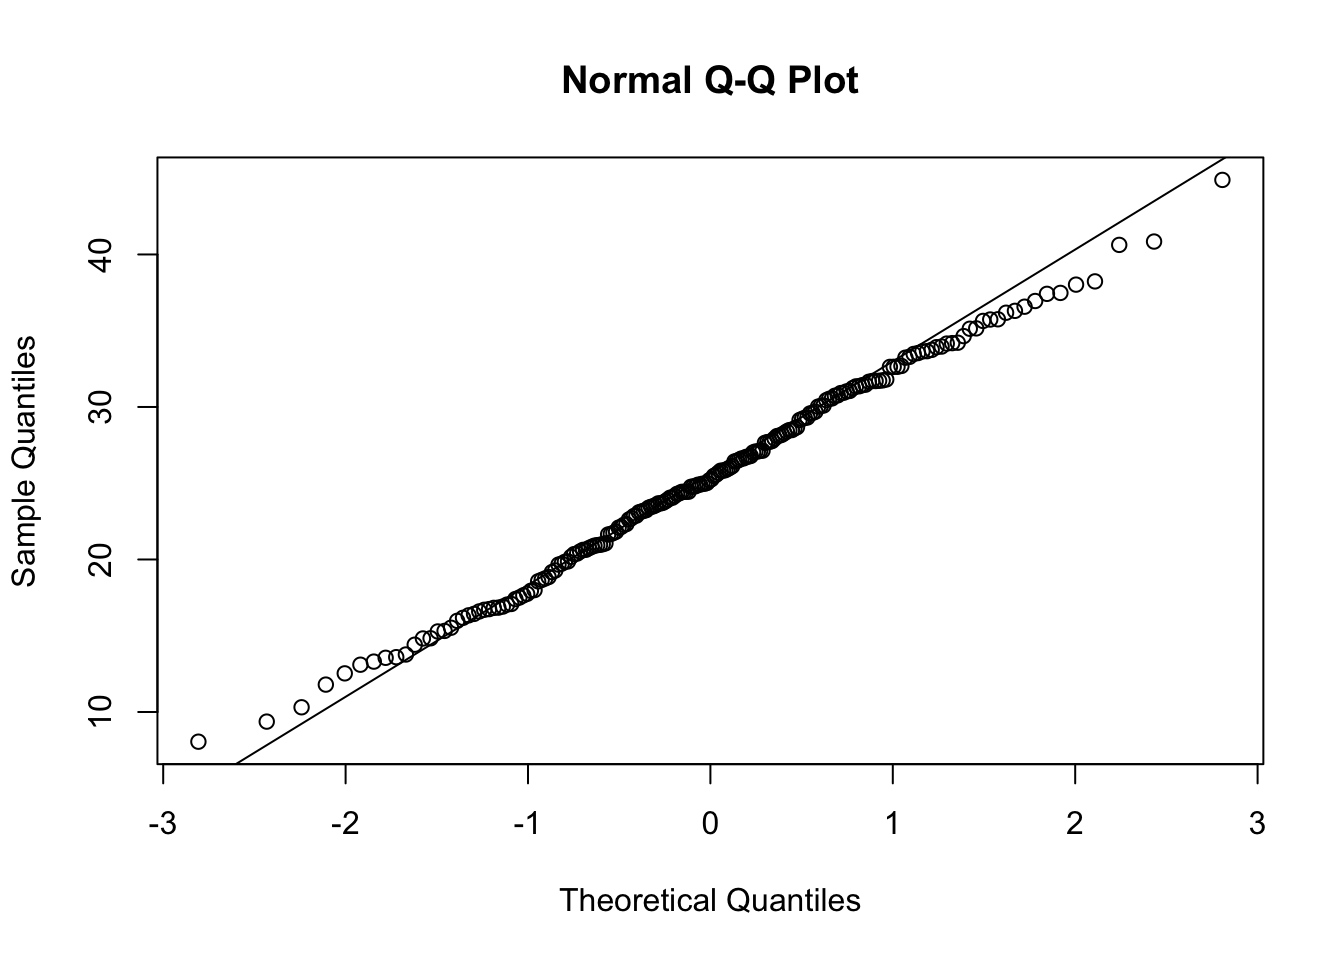
\includegraphics{test1_files/figure-latex/normality-3.pdf}

From visual inspection, BMI seems to be pretty normally distributed. But, we can also check using a more formal statistical test, the Shapiro-Wilk's test.

\begin{Shaded}
\begin{Highlighting}[]
\CommentTok{#Perform Shapiro-Wilk normality test (from base stats package)}
\KeywordTok{shapiro.test}\NormalTok{(full.data}\OperatorTok{$}\NormalTok{BMI);}
\end{Highlighting}
\end{Shaded}

\begin{verbatim}
## 
##  Shapiro-Wilk normality test
## 
## data:  full.data$BMI
## W = 0.99617, p-value = 0.9014
\end{verbatim}

We get a p-value of .9014, so cannot reject the null hypothesis. This means that we can assume normality of this data.

\hypertarget{t-tests}{%
\subsection{T-tests}\label{t-tests}}

T-tests are used to test for a significant difference between the means of two groups. There are a few types of t-tests, but here, we will be comparing BMI between two groups, smokers and non-smokers, and will be using a two sample t-test (or independent samples t-test).

TALK ABOUT ASSUMPTIONS\ldots{}

\begin{Shaded}
\begin{Highlighting}[]
\CommentTok{#It is nice to visualize the data across groups using things like boxplots}
\KeywordTok{boxplot}\NormalTok{(}\DataTypeTok{data=}\NormalTok{full.data, BMI }\OperatorTok{~}\StringTok{ }\NormalTok{Smoker);}
\end{Highlighting}
\end{Shaded}

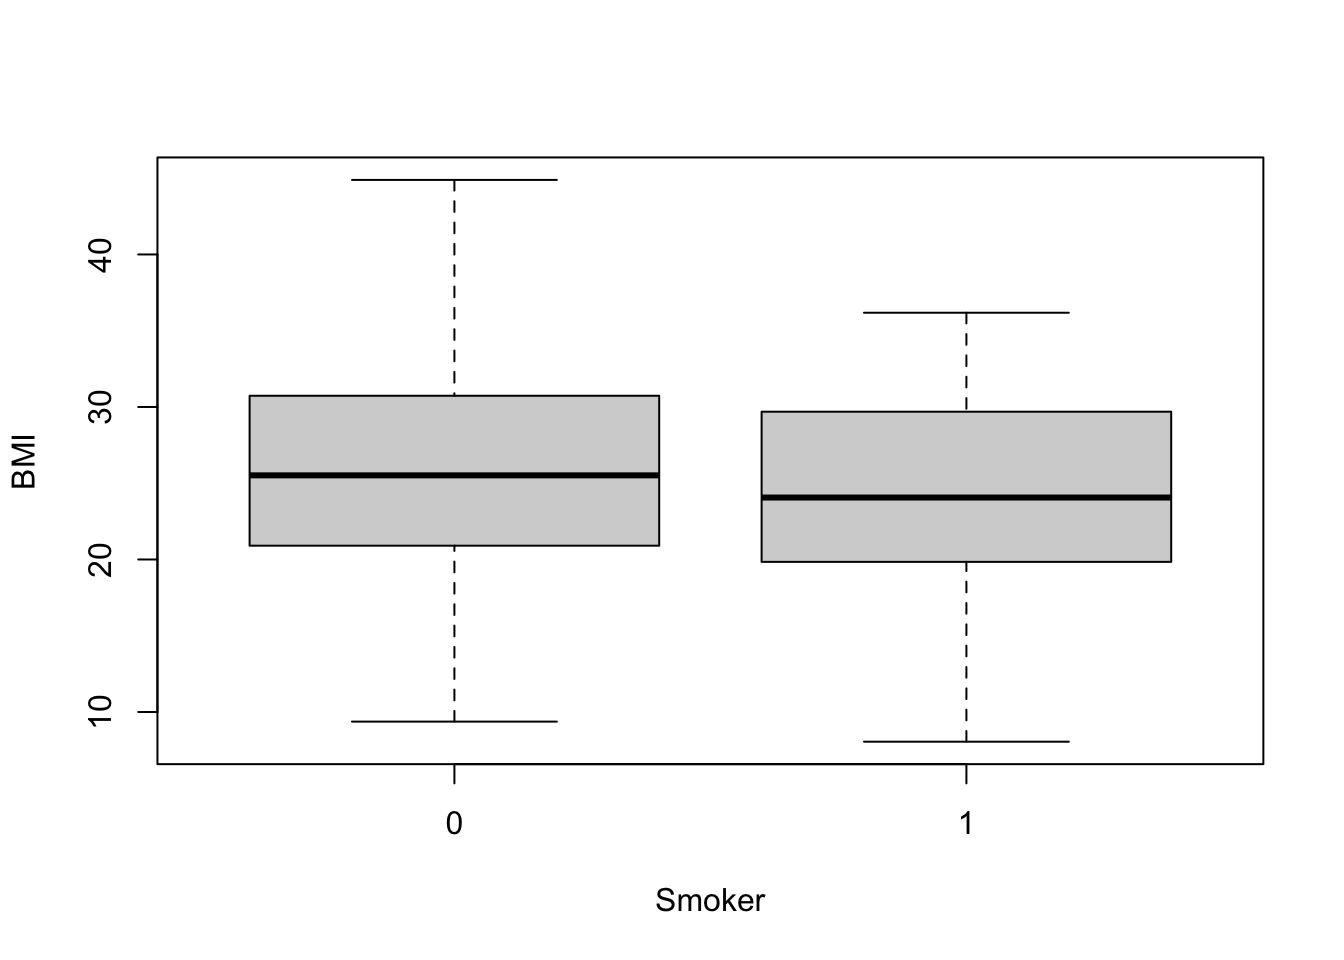
\includegraphics{test1_files/figure-latex/ttest-1.pdf}

\begin{Shaded}
\begin{Highlighting}[]
\CommentTok{#It is easy to peform a t-test on these data using t.test() from base stats package}
\KeywordTok{t.test}\NormalTok{(}\DataTypeTok{data=}\NormalTok{full.data, BMI }\OperatorTok{~}\StringTok{ }\NormalTok{Smoker);}
\end{Highlighting}
\end{Shaded}

\begin{verbatim}
## 
##  Welch Two Sample t-test
## 
## data:  BMI by Smoker
## t = 2.1275, df = 96.269, p-value = 0.03593
## alternative hypothesis: true difference in means is not equal to 0
## 95 percent confidence interval:
##  0.1431141 4.1270354
## sample estimates:
## mean in group 0 mean in group 1 
##        25.92961        23.79453
\end{verbatim}

\begin{Shaded}
\begin{Highlighting}[]
\CommentTok{#We can also save the results into a variable and access various output values}
\NormalTok{ttest.res =}\StringTok{ }\KeywordTok{t.test}\NormalTok{(}\DataTypeTok{data=}\NormalTok{full.data, BMI }\OperatorTok{~}\StringTok{ }\NormalTok{Smoker);}

\CommentTok{#For example, we can access the p-value}
\NormalTok{ttest.res}\OperatorTok{$}\NormalTok{p.value;}
\end{Highlighting}
\end{Shaded}

\begin{verbatim}
## [1] 0.03593188
\end{verbatim}

From the boxplots, it's clear that there are differences in the BMIs between smokers and non-smokers. And, in fact, when running the t-test, we see that means across groups are not equal.

\hypertarget{anova}{%
\subsection{ANOVA}\label{anova}}

Analysis of Variance (ANOVA) is a statistical method that is used to compare means of more than two groups.

TALK ABOUT ASSUMPTIONS and other stuff.

\begin{Shaded}
\begin{Highlighting}[]
\CommentTok{#Boxplots to look at data across groups}
\KeywordTok{boxplot}\NormalTok{(}\DataTypeTok{data=}\NormalTok{full.data, BMI }\OperatorTok{~}\StringTok{ }\NormalTok{Smoker3);}
\end{Highlighting}
\end{Shaded}

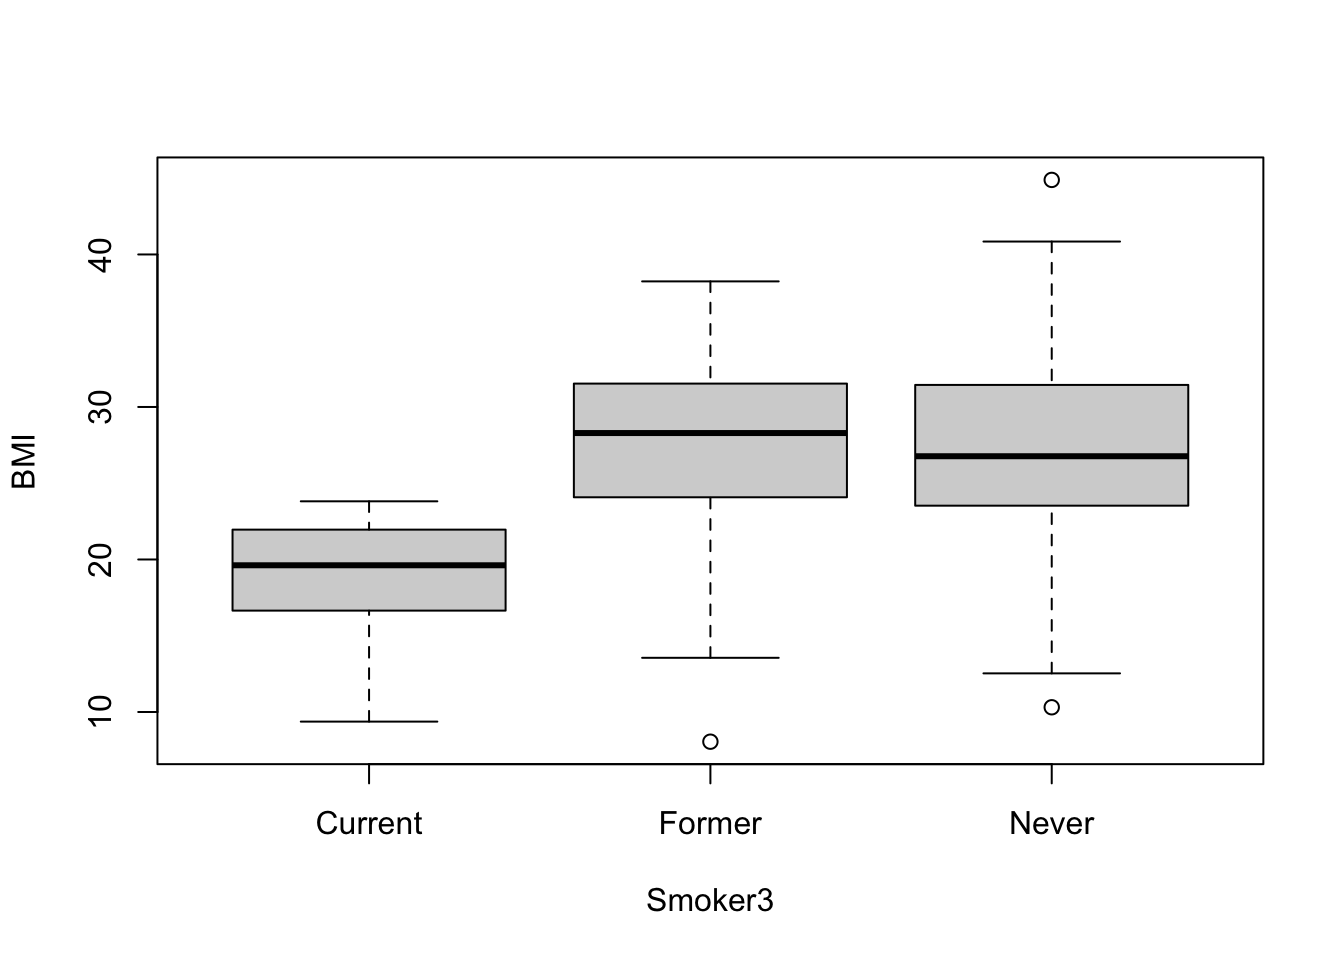
\includegraphics{test1_files/figure-latex/anova-1.pdf}

\begin{Shaded}
\begin{Highlighting}[]
\CommentTok{#Can also get group means}
\NormalTok{full.data }\OperatorTok\StringTok{ }\KeywordTok{group_by}\NormalTok{(Smoker3) }\OperatorTok\StringTok{ }\KeywordTok{summarise}\NormalTok{(}\KeywordTok{mean}\NormalTok{(BMI));}
\end{Highlighting}
\end{Shaded}

\begin{verbatim}
## # A tibble: 3 x 2
##   Smoker3 `mean(BMI)`
##   <chr>         <dbl>
## 1 Current        19.2
## 2 Former         27.7
## 3 Never          26.8
\end{verbatim}

\begin{Shaded}
\begin{Highlighting}[]
\CommentTok{#Use ANOVA to compare groups (use aov to fit ANOVA model)}
\KeywordTok{aov}\NormalTok{(}\DataTypeTok{data=}\NormalTok{full.data, BMI }\OperatorTok{~}\StringTok{ }\NormalTok{Smoker3);}
\end{Highlighting}
\end{Shaded}

\begin{verbatim}
## Call:
##    aov(formula = BMI ~ Smoker3, data = full.data)
## 
## Terms:
##                  Smoker3 Residuals
## Sum of Squares  1967.516  7250.059
## Deg. of Freedom        2       197
## 
## Residual standard error: 6.066492
## Estimated effects may be unbalanced
\end{verbatim}

\begin{Shaded}
\begin{Highlighting}[]
\CommentTok{#We can get the typical ANOVA table using either summary or anova on fitted object}
\KeywordTok{anova}\NormalTok{(}\KeywordTok{aov}\NormalTok{(}\DataTypeTok{data=}\NormalTok{full.data, BMI }\OperatorTok{~}\StringTok{ }\NormalTok{Smoker3));}
\end{Highlighting}
\end{Shaded}

\begin{verbatim}
## Analysis of Variance Table
## 
## Response: BMI
##            Df Sum Sq Mean Sq F value    Pr(>F)    
## Smoker3     2 1967.5  983.76  26.731 5.357e-11 ***
## Residuals 197 7250.1   36.80                      
## ---
## Signif. codes:  0 '***' 0.001 '**' 0.01 '*' 0.05 '.' 0.1 ' ' 1
\end{verbatim}

From the ANOVA table, we can conclude that the group means are not all equal.

\hypertarget{regression-linear-regression-and-logistic-regression}{%
\subsection{Regression: linear regression and logistic regression}\label{regression-linear-regression-and-logistic-regression}}

\hypertarget{chi-squared-test-box-plots}{%
\subsection{Chi-squared test -- box plots}\label{chi-squared-test-box-plots}}

\hypertarget{fishers-exact-test}{%
\subsection{Fisher's exact test}\label{fishers-exact-test}}

\hypertarget{heat-maps}{%
\section{Heat maps}\label{heat-maps}}

\hypertarget{pheatmap}{%
\subsection{pheatmap}\label{pheatmap}}

\hypertarget{heatmap2}{%
\subsection{heatmap2}\label{heatmap2}}

\hypertarget{superheat}{%
\subsection{superheat}\label{superheat}}

\hypertarget{clustering}{%
\section{Clustering}\label{clustering}}

Examples with genomics: Rager et al.~2014

\hypertarget{hierarchical}{%
\subsection{Hierarchical}\label{hierarchical}}

\hypertarget{k-means}{%
\subsection{K-means}\label{k-means}}

\hypertarget{data-reduction-pca}{%
\section{Data reduction (PCA)}\label{data-reduction-pca}}

\hypertarget{visualize-pca-plot}{%
\subsection{Visualize PCA Plot}\label{visualize-pca-plot}}

\hypertarget{identify-of-variance-captured}{%
\subsection{Identify \% of variance captured}\label{identify-of-variance-captured}}

\hypertarget{multi-omics-analyses-for-environmental-health}{%
\chapter{Multi-Omics Analyses for Environmental Health}\label{multi-omics-analyses-for-environmental-health}}

\hypertarget{exposomics}{%
\section{Exposomics}\label{exposomics}}

\hypertarget{placenta-exposome}{%
\subsection{Placenta Exposome}\label{placenta-exposome}}

about to be submitted to EI
Dust NTA data

\hypertarget{transcriptomics}{%
\section{Transcriptomics}\label{transcriptomics}}

\hypertarget{deseq2-rnaseq}{%
\subsection{DESeq2 / RNAseq}\label{deseq2-rnaseq}}

Wildfire dataset, available through GEO

\hypertarget{genome-wide-microrna}{%
\section{Genome-wide MicroRNA}\label{genome-wide-microrna}}

Rager et al.~2014 miRNAs

\hypertarget{genome-wide-dna-methylation}{%
\section{Genome-wide DNA Methylation}\label{genome-wide-dna-methylation}}

\hypertarget{illumina-array-data}{%
\subsection{Illumina array data}\label{illumina-array-data}}

\begin{verbatim}
https://www.ncbi.nlm.nih.gov/geo/query/acc.cgi?acc=GSE58499
https://www.ncbi.nlm.nih.gov/geo/query/acc.cgi?acc=GSE28368
\end{verbatim}

\hypertarget{proteomics}{%
\section{Proteomics}\label{proteomics}}

\begin{verbatim}
Bailey et al arsenic dataset maybe?
\end{verbatim}

\hypertarget{mixtures-analyses-for-environmental-health}{%
\chapter{Mixtures Analyses for Environmental Health}\label{mixtures-analyses-for-environmental-health}}

\hypertarget{sufficient-similarity}{%
\section{Sufficient Similarity}\label{sufficient-similarity}}

Botanicals example with chemistry and tox profiling -- Julia has dataset

\hypertarget{mixtures-modeling-through-qgcomp}{%
\section{Mixtures Modeling through qgcomp}\label{mixtures-modeling-through-qgcomp}}

Could use published wildfire analysis here (Rager et al.~2021, STOTEN), or online example provide through Alex Keil's studies

\hypertarget{environmental-health-databases}{%
\chapter{Environmental Health Databases}\label{environmental-health-databases}}

\hypertarget{comparative-toxicogenomics-database-ctd}{%
\section{Comparative Toxicogenomics Database (CTD)}\label{comparative-toxicogenomics-database-ctd}}

\hypertarget{gene-expression-omnibus-geo}{%
\section{Gene Expression Omnibus (GEO)}\label{gene-expression-omnibus-geo}}

\hypertarget{nhanes}{%
\section{NHANES}\label{nhanes}}

\end{document}
